\section{Main result: early plausibility, late commitment}

Figure~\ref{fig:flagship} is the central result of the paper. The two cumulative curves are far apart. By 20\% of normalized depth, the eventual answer is already plausible for \FlagshipTwentyPlausiblePct{} of evaluable cases, but it is already committed for only \FlagshipTwentyCommittedPct{}. The gap stays large through the middle of the network. At 50\% of normalized depth, \FlagshipFiftyPlausiblePct{} of evaluable cases have already admitted the eventual answer into the plausible set, while only \FlagshipFiftyCommittedPct{} have already reached stable commitment. In raw layer units, the pooled grouped-bootstrap median commitment lag is \PooledLagMedian{} layers with a 95\% confidence interval of [\PooledLagCILow{}, \PooledLagCIHigh{}].

The dataset panels show that this is not coming from just one benchmark. ARC-Challenge
and CommonsenseQA both show the same broad shape: plausibility rises early, while
commitment stays much lower until later in depth. So the pooled result is not an artifact
of one dataset or one model family.

\begin{figure*}[t]
\centering
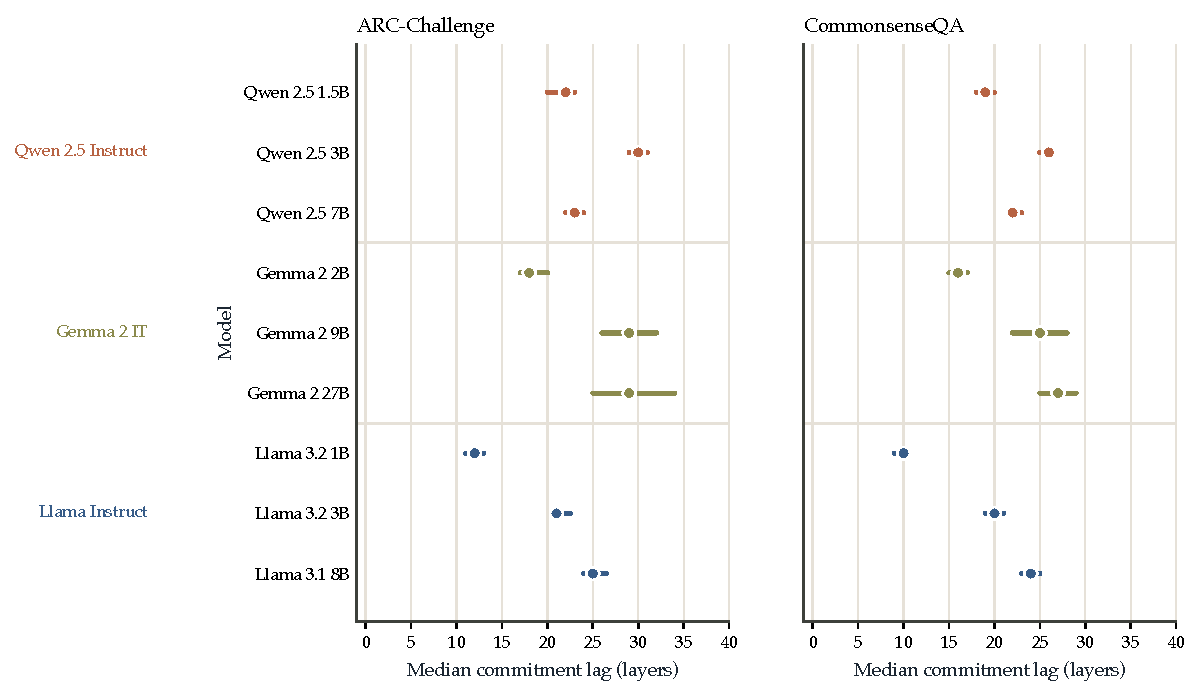
\includegraphics[width=\textwidth]{figure2_primary_forest_plot.pdf}
\caption{\textbf{Every evaluable ARC-Challenge and CommonsenseQA cell is positive under the preregistered primary rule.} Each point is the cell-level median commitment lag $\Delta_{\mathrm{margin}}$ in raw layer units for the primary analysis path, and each horizontal interval is a grouped-bootstrap 95\% confidence interval. Every reported model-dataset cell is positive.}
\label{fig:forest}
\end{figure*}

Figure~\ref{fig:forest} and Table~\ref{tab:primary-summary} translate the pooled picture
into the preregistered cell-level decision rule. All \ArcCsqaPositiveCells{} evaluable
ARC-Challenge and CommonsenseQA cells are positive, and there are no evaluated
negatives. So the main pattern is not just a pooled average. It survives at the level of
individual model-dataset cells.

\begin{table}[t]
\centering
\small
\begin{tabular}{@{}lccc@{}}
\toprule
Dataset & Positive & Evaluable & Insufficient \\
\midrule
ARC-Challenge & 9 & 9 & 0 \\
CommonsenseQA & 9 & 9 & 0 \\
All reported datasets & 18 & 18 & 0 \\
\bottomrule
\end{tabular}

\caption{\textbf{Primary-rule summary by dataset.} ARC-Challenge and CommonsenseQA are positive in every evaluable model-dataset cell.}
\label{tab:primary-summary}
\end{table}

The family-level summaries tell the same story. Qwen contributes six positive primary cells,
Gemma contributes six, and Llama contributes six. So the result is broad across the chosen
instruct-model panel, even though the exact lag size still varies with model depth and
dataset difficulty.

\FloatBarrier
